\documentclass[a4paper, oneside]{ipsreport}

\usepackage[utf8]{inputenc}
\usepackage[T1]{fontenc}
\usepackage[sc]{mathpazo} % Use the Palatino font
\usepackage[american]{babel} % Language hyphenation and typographical rules
\usepackage[toc,page]{appendix}
\usepackage{graphicx}
\onehalfspacing

\usepackage{csquotes}
\usepackage[backend=biber, style=mla, citestyle=mla, autocite=footnote]{biblatex}
\addbibresource{./references.bib}

\setlist[itemize]{noitemsep} % Make itemize lists more compact
\setlength{\parindent}{0pt}

\title{A Bluetooth Low Energy-Based Indoor Positioning System}

% \thesistype{Submission to the SJF National Competition}
\thesistype{Matura paper}

\author{Mark Marolf}

\email{mark.marolf@students.ksba.ch}

\keywords{
	Bluetooth Low Energy (BLE) beacon, Path Loss Model, Indoor Positioning System, Trilateration, IoT, localization, RSSI, tracking
}
% \institute{Department G17b \\ Kantonsschule Baden}
\institute{Kantonsschule Baden}

\supervisors{Daniel Süsstrunk, Stefan Guggenbühl}

\date{\today}

\begin{document}

\frontmatter

\maketitle

\tableofcontents

\begin{abstract}
	The following paper describes the development and construction of an installable and accurate indoor positioning system (IPS) for Internet of Things applications from scratch.

	The goal of this project is to develop the hardware and software necessary to create a cheap, high-performance IPS. In this paper I describe a readily available system that automatically approximates the position of an object in an indoor environment using Bluetooth Low Energy. The theoretical background is provided first, followed by descriptions of a wide array of experiments conducted to improve the product. Next, the software and hardware development is outlined such that anyone can reproduce the results. Finally, I benchmark the system and compare it with similar IPS described in literature.

	My system makes IPS accessible for developers, since no readily available solutions existed previously. Positioning data is available to developers via an application programming interface, while the underlying algorithms are contained and abstracted. Thus IoT projects can tap into a previously inaccessible research field without high costs or installation difficulties. The IPS can run on \$5 computers without problems, is open-sourced and work with most operating systems. Positioning accuracy is reasonably good.
\end{abstract}

\mainmatter

\chapter{Introduction}
\subsubsection{Indoor Positioning Systems}
According to predictions made by McKinsey, a consulting company, the IoT will have an economic impact between \$4 trillion and \$11 trillion USD by 2025 \autocite{McKinsey}. In a large scale scramble towards ubiquitous computing, entire industries are currently being reinvented. Yet one aspect of this digital renaissance has remained elusive: Valuable location data for countless business applications can not be provided indoors. For outdoor use, GPS has been a robust and reliable provider of positioning data for over 30 years \autocite{wiki:GPS}. In closed indoor environments, such as the warehouses, hospitals or shopping malls being revolutionized by the spread of ubiquitous computing, GPS unfortunately cannot provide service. But warehouses still want to optimize the handling their goods, hospitals would like to remotely monitor the position of patients and shopping malls want to gain insights about customer flow. Thus the rising importance of cost-effective and commercially viable indoor GPS alternative has sparked interest in the research field of Indoor Positioning Systems (IPS).

\subsubsection{Technologies}
A plethora of IPS technologies have already been proposed, each entailing their own set of advantages and drawbacks. So far two technologies already embedded in most consumer devices have come the farthest. Both Bluetooth Low Energy (BLE) and WiFi show promise for use in IPS due to their low cost and widespread availability. Take for example the Contact Tracing App released by the Swiss Government, which is conceptually related to this project. It uses BLE to compute the distance between Smartphones \autocite{SwissCovid}, similarly to how this project uses distances based on BLE signals to compute positions. In that sense this project deals with many of the obstacles probably encountered by the SwissCovid app. Findings from this project therefore provide insights regarding the feasibility and accuracy of BLE based contact tracing apps.

Research groups have shown that the same technology can be used in more complex applications, such as in IPS. Aside from their widespread availability and low cost, BLE and Wifi based systems are comparatively simple in contrast to other IPS contenders (elaborated in section \ref{section:relatedWork}). Measurements of the received signal strength indicator (RSSI) of Wifi or BLE signals can be translated into positions and subsequently be used in IoT applications.

\subsubsection{Motivation}
Despite all of these great ideas put forth in research, so far the gap between the scientific and the commercial worlds has hardly been bridged. Since I am quite interested in programming and innovative technologies, I was excited by the idea of creating a general purpose IPS. Motivated by the fact that there is a large potential for IPS but few suitable practical implementation exist, I decided to contribute the time allotted for my Matura Paper to the field.

\subsubsection{Question}
This paper deals with the question, whether it is possible to create the hardware and software for an indoor positioning system from scratch. Additionally, it discusses limits to the accuracy and feasibility of indoor positioning systems, and furthermore how both can be improved in theory and practice.

The rest of this paper will be structured as follows: Chapter \ref{chapter:materialsAndMethods} discusses how the RSSI accuracy problems are solved in order to create reliable distance estimates. Next, chapter \ref{chapter:bleips} covers the system architecture that facilitates robust, real-time positioning and visualization in a web-app. The final product is finally evaluated in chapter \ref{chapter:results}, followed by a discussion of its shortcomings and benefits in chapter \ref{chapter:discussion}.

\chapter{Materials and Methods}
\label{chapter:materialsAndMethods}

\section{Selected Related Approaches}
\label{section:relatedWork}

Research on indoor positioning systems has been done on a wide range of technologies, such as Bluetooth \autocite{BLE}, ultra-wideband \autocite{UWB} magnetic field \autocite{Magnetic}, RFID \autocite{RFID}, ultrasound \autocite{Ultrasound}, Wi-Fi \autocite{IPSESP32Client} or even visible and infrared light \autocite{visiblelight}. For many technologies, cost and impracticality make them infeasible. Cheaper options such as  Wifi and BLE show more promise. In comparison to BLE, Wifi transmits fewer packets from which RSSI can be extracted. Therefore Wifi based systems tend to be less accurate than BLE \autocite{IPSESP32Client}. RSSI from both sources though tend to fluctuate, which makes it hard to compute definite, stable positions.

\subsubsection{RSSI Fingerprinting}
A common approach to solving the RSSI fluctuation problem is RSSI Fingerprinting \autocite{Fingerprinting}. In principle measured RSSI values are compared with a previously constructed RSSI map of a room to construct a position estimate. Often the comparison is helped by particle filters, deep learning and k-nearest-neighbors classification. The initially required training phase considerably reduces the practicality of fingerprinting. Also problematic are the large numbers of beacons required to get accurate estimates and the sensitivity to environmental changes.

\subsubsection{RSSI Trilateration}
A second solution makes use of the RSSI as a proxy for the distance between two BLE devices. Feeding at least three distances into a trilateration algorithm yields a position estimate \autocite{BLE}. Extended Kalman Filters (EKF) have good performance when tracking moving targets. To further improve the quality of estimations, the positions estimates determined using trilateration are fused with additional sensor data increase accuracy. Next to the BLE-RSSI trilateration setup, an accelerometer and gyroscope constructs a model of the device's movement in space to compare with the trilateration. Yet these additions increase cost and complexity because they require additional hardware. Furthermore, it was shown in \autocite{ImuTrilaterationFusion} that errors on the side of the external sensors accumulated over time, which made positions increasingly erroneous. Another shortcoming was that the initial position had to be supplied to the sensor-based algorithm, thereby reducing the overall practicality. For the aforementioned reasons a BLE-RSSI trilateration-based does not have this issue.

\subsubsection{BLE-RSSI Trilateration Accuracy}
The accuracy of conventional BLE-based IPS is nowhere near that of GPS. In a realistic hallway setup with moving targets, an average position root mean squared error (RMSE) of 1.36m was achieved in \autocite{AntennaDiversity}. The average RMSE of positions determined using trilateration in \autocite{ImuTrilaterationFusion} was 0.78m. Most of the inaccuracy compared with GPS stems RSSI noise.

To conclude lessons learned from related work, this paper will be focused on implementing a BLE-RSSI trilateration algorithm. In basic terms, RSSI measurements coming from at least three beacons as shown in figure \ref{fig:basic_outline} will be converted to distances $r_1, r_2, r_3$. The attained distances represent the radii of circles between the beacons and a device of unknown position at $P_{dev}$. To get the coordinates of $P_{dev}$, a basic approach is to compute the intersection of the three circles.

\begin{figure}[h]
	\centering
	\includegraphics[width=\linewidth]{./figures/system_diagram.pdf}
	\captionof{figure}{Basic functionality of IPS}
	\label{fig:basic_outline}
\end{figure}

\section{Log-Distance Path Loss Model}
\label{section:pathLossModel}
\subsection{Theoretical Background}
\label{subsection:theoreticalBackground}
With BLE based IPS, the function that maps the signal power to a distance forms the backbone for all subsequent calculations. An accurate model is thus essential to compute distance estimates from RSSI measurements. \autocite{AntennaDiversity} shows experimentally that the log-normal path loss model (PLM) provides an adequate statistical representation. The PLM may be expressed as
\begin{equation} \label{eq:1}
	RSSI(d) = \overline{RSSI}_{d_0} - 10n \times log_{10} (\frac{d}{d_0}) + W
\end{equation}
where $RSSI(d)$ is the received power in dBm at a distance $d$ meters from the transmitter, n is the path loss exponent which defines the rate of power attenuation with respect to distance and $W$ is a normally distributed random variable. Variables that influence $W$ are explained later on. $RSSI_{d_0}$ represents the average signal power at the distance $d_0$. For practical reasons, $d_0$ is often chosen to be 1 meter since the fraction $\frac{d}{d_0}$ is consequently equivalent to just $d$. Both $n$ and $RSSI_{d_0}$ have to be determined in advance either experimentally or using data available in literature.

The signal propagation of a BLE signal in an indoor environment is influenced by many different things. Obstacles such as humans, furniture or structural elements of the room lead to shadowing and signal absorption. Many materials also can reflect radio signals, which leads to multipath propagation and small scale fading. Changes in the antenna orientation lead further distort the power level as shown in \autocite{AntennaOrientationRssi}. These considerations are represented in the PLM using the aforementioned random variable $W$. According to \autocite{AntennaDiversity}, $W$ can thus be denoted as follows:
\begin{equation} \label{eq:2}
	W = X + S + G
\end{equation}
$X$ is regarded as the effect of small scale fading. $S$ denotes the influence of shadowing caused by the obstruction of the line of sight between devices. $G$ is a normally distributed random variable that accounts for random antenna orientations. In an ideal environment with no shadowing or fading, the influence of $X$ and $S$ is negligible, leaving us with a normally distributed random variable $\tilde{W}$ that is only influenced by $G$. Hence under optimal conditions the PLM can be expressed as
\begin{equation} \label{eq:correctedPathLossModel}
	RSSI(d) = \overline{RSSI}_{d_0} - 10n \times log(d) + \tilde{W}
\end{equation}

With this information regarding the underlying problems of the path loss model, we can move forward with the construction of the system. Much of the rest of the project is concerned with finding ways to reduce noise from fading and shadowing such that equation \ref{eq:correctedPathLossModel} is applicable. Theoretical and practical solutions to guarantee the validity of the PLM are subject of the next sections.

\subsection{Transmitting and Receiving BLE RSSI}

\subsubsection{BLE Specification}
The BLE specification defines how connections are made and ensures robust and secure data transmission. Contrarily to Wifi, the TCP/IP protocols are not used for data transmission. A BLE specific subset of rules centered around the notion of services dictates how information is shared. Take for example a BLE module that wants to share telemetry from a temperature sensor. It designates a service dedicated to the readings and tags the service with a universally unique identifier (UUID). Said service is then advertised to nearby BLE clients, that by chance might be listening for available services. If the UUID attached to a received service notice is interesting, more complex forms of interaction such as connections and BLE characteristics are initiated. BLE advertising / observing model already sufficed for this project, so nothing more complicated was pursued. Connections were finicky with the amount of beacons that could be simultaneously connected to and used more system memory.

\begin{figure}[h]
	\centering
	\includegraphics[width=\linewidth]{./figures/ble-advertiser-observer.pdf}
	\captionof{figure}{BLE advertising and observing in this IPS}
	\label{fig:ble-advertiser-observer}
\end{figure}

\paragraph{BLE advertiser}
To put in the roles of BLE advertisers and clients, I ordered ten ESP32 low-cost, low-power microcontrollers and batteries to power them from Aliexpress. Despite costing only \$6 USD, Wifi and BLE 4.2 were fully integrated into the system on a chip (SoC) \autocite{TtgoTdisplay}. I programmed the ESP32 using the C++ programming language and the Arduino-ESP32 software development core. This software development kit gave me access to various libraries concerned with managing the BLE API of FreeRTOS, the ESP32's operating system. As can be seen below, the BLE advertising code was fairly simple. It instructed the ESP32 to advertise indefinitely using settings I found to be optimal \footnote{Considerations elaborated in subsection \ref{subsection:noiseReduction}}.

\begin{lstlisting}[language=C++]
int advertisingIntervalTarget = 100;

void setupBeacon() {
	BLEDevice::init("BLE IPS Server");

	//  set tx power level to -3 dBm
	BLEDevice::setPower(ESP_PWR_LVL_N3);

	advertiser = BLEDevice::getAdvertising();
	advertiser->addServiceUUID(SERVICE_UUID);

	advertiser->setMinInterval(advertisingIntervalTarget - 20);
	advertiser->setMaxInterval(advertisingIntervalTarget + 20);
}

void setup() {
	setupBeacon();

	advertiser->start();
}
\end{lstlisting}

While the beacons above advertise data at the highest feasible rate possible, BLE clients listen to BLE channels dedicated to the IPS and collect RSSI measurements. Using the ESP32's integrated Wifi, I initially intended to put them in the role of thin clients and directly relay RSSI over Wifi to the backend. I spent roughly a month programming the aforementioned client. Despite having working code for the BLE part and working asynchronous HTTP webservices that could send data wirelessly my backend, I couldn't get around memory management issues. The ESP32 has only 320 Kb of RAM, so I could not simultaneously load the BLE and HTTP code into memory. For comparison, the computer I am typing this sentence on has 100'000 times more memory. After spending a month tinkering with solutions to get around the acute lack of memory, I gave up and switched to a few variants of the Raspberry Pi.

The Raspberry Pi platform was implemented using Node.js and an open-source BLE library called Noble.js. Technically it had cross-platform support, but on Windows only certain BLE adapters worked correctly due to the way Noble.js interfaced with the host machine's HCI socket. I ignored the shortcoming and programmed a client in Typescript. RSSI measurements are aggregated and stored temporarily in a local queue. After a predetermined time the queue is uploaded to the server and cleared thereafter. The core functionality can be showcased in the following 11 lines of code:

\begin{lstlisting}[language=JavaScript, caption=IPS Client Core Functionality]
BLEController.on('stateChange', (state: any) => {
    if (state === 'poweredOn') {
        scanForDevices()

        setInterval(() => {
            if (measurementQueue.queue.length) {
                measurementQueue.uploadAndClear();
            }
        }, 250);
    }
});

\end{lstlisting}

After being received by the IPS client, measurements were sent to a remote server as JSON objects using HTTP POST requests. They were evaluated and stored on a remote server. Processing was done to reduce noise from fading and shadowing, as mentioned previously in section \ref{section:pathLossModel}.

\section{Noise reduction}
\subsection{RSSI Analysis}
To analyze RSSI variations, I collected 50 RSSI at a distance of 1m between the BLE devices. This experiment was repeated with five beacons at 20 different distances. Figure \ref{fig:rssifluctuation} shows an exemplary input stream in blue and post-processed results in red. The mean RSSI was -60.5 dBm with a standard deviation of 1.15dBm. Next, figure \ref{fig:rssiDistribution} displays a histogram of 315 RSSI measurements received from five beacons at 2.75 meters distance with a constant antenna orientation. The overall mean $\mu_{tot}$ was -65.1 dBm and the standard deviation of the RSSI under presence of fading and shadowing amounted to $\sigma_{W}$ = 6.29 dBm. Figure \ref{fig:rssiDistribution} distribution features three peaks and an overall negative skew. Under the absence of $G$ since the antenna direction remained constant, the empirical PDF of $W = S + X$ results in a Rician or Rayleigh distribution \autocite{AdvertisingInterval}. Clearly, unmodified RSSI values are not reliable enough for localization, and countermeasures are necessary to improve the usability of the RSSI values.
\begin{figure}[h!]
	\centering
	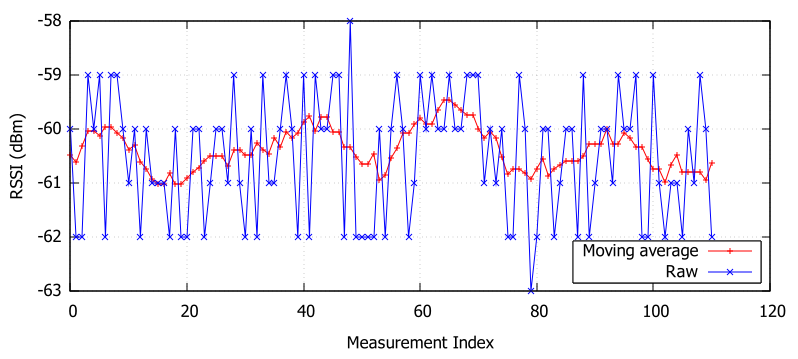
\includegraphics[width=0.7\linewidth]{./figures/rssifluctuation.pdf}
	\captionof{figure}{RSSI fluctuations}
	\label{fig:rssifluctuation}
	\includegraphics[width=0.7\linewidth]{./figures/rssiDistribution.pdf}
	\caption{Histogram of 315 RSSI under influence of shadowing and fading}
	\label{fig:rssiDistribution}
\end{figure}

\subsection{Noise Reduction in Practice}
\label{subsection:noiseReduction}
This section is concerned with limiting the impact of multipath fading and shadowing. In total I conducted over 70 experiments \footnote{See data availability statement in appendix \ref{appendix:rssimeasurementdata}} to test ideas that helped increase the usability of RSSI. Noise reduction was most effectively achieved by increasing the signal diversity order for BLE channels. Other attempts at improvement were mostly incremental.

\subsubsection{Hardware-based Solutions}
My first approach was to elevate the BLE devices (height $\approx 1m$) off the ground using custom-built stands, such that a constant line of sight between BLE devices is maintained. This reduces the effect of shadowing, caused by obstructions of the line of sight. Since this sort of equipment is not available commercially, I first had to build the setup myself. The modules were mounted on stands using custom-designed 3D printed cases\footnote{3D printable Gcode and STL files are available in appendix \ref{appendix:3dfiles} }. 3D models were constructed in Tinkercad and sliced in Cura. The Raspberry Pi case showcased in figure \ref{fig:multiclient} went through six design iterations. It fits all generations of Raspberry Pi and was specifically designed for use in an IPS in mind. Figure \ref{fig:beacon} displays the final beacon case after seven design iterations.

\begin{figure}[h]
	\begin{minipage}{.5\textwidth}
		\centering
		\includegraphics[width=0.95\linewidth]{./figures/raspi4.png}
		\captionof{figure}{Raspberry Pi 4 Model B}
		\label{fig:raspi4modelb}
	\end{minipage}
	\begin{minipage}{.5\textwidth}
		\centering
		\includegraphics[width=0.95\linewidth]{./figures/beacon.jpg}
		\captionof{figure}{ESP32 BLE beacon}
		\label{fig:beacon}
	\end{minipage}
\end{figure}

The materials used (PLA plastic and wood) were selected as they do not absorb radiation at 2.4 GHz. Cutouts in the PLA ensured that antennae were left unobstructed. Because radiation was emitted outwards, perpendicular to the printed circuit board, all antennae were mounted vertically. Radiation patterns thus mostly uniform and omnidirectional, further reducing the normal perturbation $G$ caused by random antenna orientations of the transmitter and receiver. The device's antenna were raised above the case as not to be obstructed by the case or battery, which would have caused shadowing. Furthermore, metal objects that couldn't be removed (wires, batteries) were kept away from the antennae. In an experiment conducted to quantify the resulting improvement, the standard deviation of 50 RSSI values was reduced by 53\% from $\sigma_W$ = 7.06 dBm to $\sigma_W$ = 3.37 dBm.

Another hardware-based form of noise reduction was the inclusion of spatial diversity in BLE channels. This involves separating antennae by at least half a wavelength ($\lambda \approx 12cm$). Increasing diversity in wireless communications is a method for improving the reliability of a communication channel. It provides two or more inputs at the BLE receiver such that the noise of these is unrelated and can be exploited in multiple dimensions simultaneously. \autocite{AntennaDiversity} showed by including one or more forms of signal diversity, the RMSE can be reduced significantly such that channel fading is negligible. It concluded that 3 or 4 diversity branches were enough to neglect small-scale fading. Spatial diversity was achieved in practice by positioning three antennae in a triangular constellation on a plane roughly 25cm apart as shown in \ref{fig:multiclient}. This shape allows for spatial separation along both coordinate grid axes and a symmetrical weight distribution.

\begin{figure}[h]
	\centering
	\begin{minipage}{.75\textwidth}
		\centering
		\includegraphics[width=\linewidth]{./figures/multiclient.jpg}
		\captionof{figure}{Raspberry Pi BLE clients in multiclient configuration}
		\label{fig:multiclient}
	\end{minipage}%
\end{figure}

For this setup, a special PLA structural element was created in CAD and printed to split the stand mounting points three ways. Furthermore, a stable movable base with wheels was constructed to ensure mobility despite the increasingly unwieldy setup. Apart from higher loads on structural elements, the backend software had to be refactored to cope with triple the amount of measurement data \footnote{This is described with greater detail in section \ref{section:systemarchitecture}}.

\subsubsection{Software-based Solutions}
\paragraph{Rolling Averages}
Further diversity was achieved by applying an unweighted rolling average to RSSI values subject to the same shadowing, antenna gain and path loss. This creates diversity both in time and in frequency due to the way the BLE specification manages data transmission. The BLE advertiser, or concretely the ESP32, switches randomly between three discrete frequency levels by design \autocite{Esp32GAP}. Combining multiple inputs at the BLE receiver exploits temporal and spectral diversity. More sophisticated forms of algorithmic filtering such as Extended Kalman Filtering and Hampel Filtering to remove outliers were initially slated for implementation. Unfortunately these could not be introduced due to time constraints.

A wave of tests was dedicated to finding an optimal window size for the averaging filter. According to the Central Limit Theorem, large window sizes more adequately approximate the true power level. The tradeoff to large windows are high latency necessary to collect data for a moving average and decreased reactivity to client movements. An optimal window size of 11 measurements per antenna suggested by \autocite{BayesianFiltering} was confirmed experimentally. Standard deviations were acceptably low while still detecting abrupt changes in client position. Later experiments also showed that linearly scaling the window size according to the number of active antennae reduced the average position RMSE.

\paragraph{Advertising Intervals}
Yet another wave of 14 experiments, I observed changes caused by varying advertising intervals and transmission power levels in order to find a balance between battery longevity and signal stability. Literature suggested that higher transmission power levels constituted more stable signals \autocite{AdvertisingIntervalBestPractices}. Findings further elaborated in \autocite{AdvertisingInterval} inferred that short advertising intervals resulted in smaller RSSI standard deviations. In practice I found that the highest transmitter power levels indeed increased signal stability, yet drained the 2000 mAh LiPo batteries prohibitively fast. Especially since commercially available BLE beacons are operated using coin cell batteries, the highest power levels did not realistically represent realistic use cases. In total I evaluated  over 18'975 measurements automatically using Python and GnuPlot scripts to confirm the statistical inference. To conclude, my findings stated that 100ms advertising intervals showed similar levels of accuracy to the minimum of 20ms while still allowing for two days of battery runtime on a single charge.

\paragraph{Frequency Band Change for Data Transmission}
Since BLE and conventional Wi-Fi type occupied the same frequency band at 2.4 GHz, potential for interference existed. Therefore it was important to see if Wi-Fi and BLE could coexist, otherwise the reliability of RSSI might have been affected. Guided by this idea, I investigated a switch to the 5 GHz Wi-Fi band for data transmission. This reduced the standard deviation of RSSI measurements by almost 90\%. The average standard deviation when sending 398 RSSI over conventional 2.4 GHz was 3.2 dBm. This number dropped to 0.34 dBm when 438 measurements were sent over a 5 GHz network. Switching to a different Wi-Fi frequency band was equivalent in experiments to evaluating RSSI directly on the same host machine. In that sense, a frequency switch amounted to the same situation as if there were no network traffic in the first place. Nonetheless, in relative terms the benefit of using 5 GHz Wifi was not as impressive as it first seemed. Even though the changes were generally statistically significant, the overall reduction in the standard deviation was still small relative to the mean RSSI. To further dampen the significance of the gains, external references such as \autocite{WifiBluetoothInterferenceMathworks, WifiBluetoothInterferenceApple} cited interference only in certain situations, while \autocite{BLEWifiCoexistence} goes as far to claim there is no interference at all. This inconclusiveness meant that more effective noise reduction methods had to be investigated.

\paragraph{Real-Time RSSI Correction}
Additionally, I implemented and unit-tested a promising real-time correction algorithm proposed in \autocite{GatewayClient} in PHP. Said algorithm required an additional gateway BLE client of constant position. The gateway's task was to measure RSSI independently and additionally to the mobile client. The RSSI fluctuations caused by changes in the BLE beacons' transmission power level would consequently have been picked up by both the gateway and the client. Since the resulting deviations from the mean caused by power fluctuations should have been equal on both devices, the gateway data could have correct the client RSSI in real-time. For each RSSI measurement collected by the gateway stemming from Beacon $B_i$, the RSSI $R_{G_i}$ was subtracted from the unweighted log-scaled average gateway RSSI $\overline{R_{G_i}}$ such that
\begin{equation} \label{eq:gatewayClientBeacon}
	R_{G_i} - \overline{R_{G_i}} = \Delta A_i
\end{equation}
where $\Delta A_i$ represented the real-time deviation from the mean caused by power level fluctuation. $\Delta A_i$ was used as a correction offset to be applied to client RSSI measurements coming from the same beacon, which resulted in
\begin{equation} \label{eq:correctionOffset}
	R_{C_i} - \Delta A_i = \tilde{R}_{C_i}
\end{equation}
with $\tilde{R}_{C_i}$ being the real time corrected client RSSI. Every measurement was timestamped in order to match up closest gateway and client measurements timewise. To ensure accurate timestamping, a NTP server in the local area network provided all clients with network time accurate to $\pm 1000 \mu s$

The problem with this strategy was that I found no positive correlation between the values picked up by the gateway and client that could be attributed to transmitter power level fluctuations. For various advertising interval and power level settings, no positive correlation could be found that made this strategy applicable. Consider figure \ref{fig:realtimecorrection}: There is no discernible link between the curve progression of the client and the gateway. For that reason, no real time corrections could be made using gateway RSSI data, since they were not linked to the client side measurements. Quantitatively, the real-time correction was also experimentally proven to be futile. The standard deviations of the corrected client RSSI were consistently higher than the unchanged client values. In that sense the real-time correction was often more inaccurate than the unchanged value. For this reason the real-time correction algorithm was scrapped.
\begin{figure}[h!]
	\centering
	\includegraphics[width=\linewidth]{./figures/realtimecorrection.pdf}
	\captionof{figure}{Real Time RSSI Correction}
	\label{fig:realtimecorrection}
\end{figure}

\newpage
\section{Calibration}
Subsection \ref{subsection:noiseReduction} focused on the reduction of noise in RSSI measurements. In this subsection, these filtered values are converted to distances using the PLM. In terms of the project outline given by figure \ref{fig:basic_outline}, I want to draw circles of the right size around beacons. To recall, the corrected PLM defined in equation \ref{eq:correctedPathLossModel} needs to be supplied with a path loss exponent $n$ and the average power received at 1 meter as $\overline{RSSI}_{d_0}$. The former coefficient determines the rate of signal attenuation based on distance and the latter defines a reference RSSI value at 1m. With these coefficients in place, I can transform an RSSI value $RSSI_D$ into a distance  corresponding to the radius of the circles in figure \ref{fig:basic_outline} using the equation
\begin{equation} \label{eq:distanceformula}
	d = 10^{\frac{\overline{RSSI}_{d_0} - RSSI_D}{-10 \cdot n}}
\end{equation}
Because BLE signal propagation does not behave the same in different environments, globally determined coefficients are not suitable for indoor positioning. Extensive experiments showed that every beacon had a unique set of PLM coefficients and that these changed gradually over time. Room properties such as size, amount of furniture and humans, location of the beacons or external BLE traffic influenced signal propagation. Figure \ref{fig:pathlossmodel} displays how different the PLM coefficient were for eight beacons, despite being in the same room. Since the PLM is a logarithmic function, the first derivative is monotonously decreasing and tends towards 0 when the distances $d$ are very large. Hence for increasingly large $d$, the difference in power level is intrinsically very small. Therefore a difference of merely $\pm 2 dBm$ for example can result in disproportionately large distance estimate errors. Especially since the resulting PLM distance estimates serve as the foundation for further calculations, I had to determine the underlying coefficients accurately and efficiently to ensure precise results.
\begin{figure}[h]
	\centering
	\includegraphics[width=\linewidth]{./figures/plm.pdf}
	\captionof{figure}{Unique Path Loss Model Coefficients}
	\label{fig:pathlossmodel}
\end{figure}

\newpage
\subsection{Calibration Implementation}
I collected calibration data to represent the signal propagation environment in subsequent linear regression. In practice, I determined this data in advance for every single beacon through manual calibration. I laid a tape measure towards the center of the room. This increased the likelihood that the data collected for the given antenna orientation would be representative of other orientations towards the corners. Next, a client-side script guided me through the calibration steps at known, predetermined distances. Initially I set these set to 0.25m intervals, but changed them later on since data collection at such granular increments proved to be very time consuming. Hence, between 0.5m and 4m, data was automatically collected for five seconds in only 0.5m intervals. Afterwards they were uploaded to the IPS. Once again, the practical implementation in Typescript can be understood from the main function that coordinates subroutines. Note that beacons in the code are designated as server objects. This is because I initially found it a more apt description of the BLE module's role in BLE signal transmission, since it technically serves data and the client consumes it as is the case in conventional server-client constellations. Obviously in this context this denotation is confusing since the term server is often associated with web servers.

\begin{lstlisting}[language=JavaScript, caption=Calibration Function]
	async function calibrate(): Promise<void> {
		await promptUserToSelectAServerForCalibration()
		await runCalibrationSteps()

		await webservice.storeMeasurementQueue(measurementQueue.queue);
		await webservice.calibrateServer(selectedServer);

		process.exit(0);
	}
\end{lstlisting}


Like this I automatically collected roughly 1'100 measurements for every beacon and tagged them with the distance at which they were taken. Using linear regression preceded by a logarithmic transformation of the distances, I conducted a curve fit on the calibration data. Since the coefficients were found using least-squares fitting, the values could be determined directly \autocite{WolframAlpha}. For a set of $k$ measurements such that each element consisted of a RSSI value $R_i$ and their corresponding distance $d_i$, the definite path loss coefficients $n$ and $\overline{RSSI}_{d_0}$ were programmatically computed via an intermediate attenuation rate $I_k$ using

\begin{equation}
	\label{eq:LSFforcoefficients}
	\begin{split}
		I_k &= \frac{k \sum_{i=1}^k (R_i \cdot \log_{10}{d_i}) - \sum_{i=1}^k R_i \cdot \sum_{i=1}^k \log_{10}{d_i}} {k \sum_{i=1}^k (\log_{10}{d_i})^2 - (\sum_{i=1}^k \log_{10}{d_i})^2} 	\\
		\overline{RSSI}_{d_0} &=  \frac{\sum_{i=1}^k (R_i) - I_k \cdot \sum_{i=1}^k (\log_{10}{d_i})}{I_k}	\\
		n &= \frac{I_k}{-10}
	\end{split}
\end{equation}

I implemented and unit-tested this using raw PHP functions as a single PHP class \footnote{Full implementation in file \bfseries \href{https://gitlab.com/mark-matura/ble-ips-api/-/blob/master/app/Helpers/FitCalibrationData.php}{FitCalibrationData.php}}. The resulting coefficients were saved in a database for later retrieval by the trilateration algorithm or graphical user interface.

\section{Trilateration}
\label{section:trilateration}

I still have to compute the unknown position of the clients using distance estimates converted from RSSI as specified by the PLM. For this at least three reference beacons of known position have to supply distances. As already rudimentarily shown in figure \ref{fig:basic_outline}, every beacon $B_i$ forms a circle around itself with the radius $r_i$ being the distance to the client such that
\begin{equation} \label{eq:radiusofbeacon}
	r_i = (x - x_i)^2 + (y - y_i)^2
\end{equation}
The point of intersection of the three circles lies at the position coordinates (x, y) of the client. Thus, to find a hidden client, one would only have to solve the following set of equations:
\begin{equation}
\label{eq:lineartrilateration}
\begin{split}
	r_1 = (x - x_1)^2 + (y - y_1)^2 \\
	r_2 = (x - x_2)^2 + (y - y_2)^2 \\
	r_3 = (x - x_3)^2 + (y - y_3)^2 \\
\end{split}
\end{equation}
A significant problem with this approach is that it yields a single solution only when the radii are known and correct. Even in a perfect environment such as an anechoic chamber, Gaussian noise caused by random antenna orientations ($\tilde{W}$) muddies the validity of distance estimates. As such, instead of forming a single point of intersections the circles can form multiple intersections as demonstrated in figure \ref{fig:trilaterationarea} or simply not intersect at all.

\begin{figure}[h]
	\def\firstcircle{(0,0) circle (2.5cm)}
	\def\secondcircle{(3,-1) circle (2.2cm)}
	\def\thirdcircle{(3, 1.5) circle (2.75cm)}

	\centering
	\begin{tikzpicture}
		\begin{scope}
			\clip \secondcircle;
			\clip \firstcircle;
			\fill[cyan] \thirdcircle;
		\end{scope}
		\begin{scope}
			\clip \firstcircle;
			\clip \secondcircle;
			\fill[cyan] \thirdcircle;
		\end{scope}

		% draw the circles themselves
		\draw \firstcircle node[text=black,above] {$B_1$} ;
		\draw \secondcircle node [text=black,above] {$B_2$};
		\draw \thirdcircle node [text=black,above] {$B_3$};

		% draw dots at midpoints of the circles
		\draw (0, 0)  circle (0.05cm);
		\draw (3, -1)  circle (0.05cm);
		\draw (3, 1.5) circle (0.05cm);

		% draw radii
		\draw (0, 0) -- (-2.5, 0)  node[text=black,midway,below] {$r_1$} ;
		\draw (3, -1) -- (5.25, -1) node[text=black,midway,above] {$r_2$} ;
		\draw (3, 1.5) -- (5.75, 1.5) node[text=black,midway,above] {$r_3$} ;

	\end{tikzpicture}
	\caption{"Solution Area" Caused by Imperfect Distance Estimates}
	\label{fig:trilaterationarea}
\end{figure}
Programmatically handling all possible combinations of intersection caused by distance over- and underestimation is tedious. Other ideas, such as calculating the centroid of the intersection points are computationally expensive and do not cover all conditions. The most complete solution to this problem is to minimize the residuals $\rho_i$ for all beacons such that the difference between the computed distances $r_i$ and estimated distances $e_i$ is minimized \autocite{localizationMIT} in the form of an optimization problem.
\begin{equation}
	\label{eq:residual}
	\begin{split}
		\rho_i & =  r_i - e_i \\
			& = r_i^2 - (x - x_i)^2 - (y - y_i)^2
	\end{split}
\end{equation}
Assuming high enough signal diversity orders are achieved and the effect of small scale fading and shadowing are successfully eliminated such that the corrected PLM equation \ref{eq:correctedPathLossModel} is applicable, a Gaussian distribution can be assumed. Hence I obtained the PLM-based position using the maximum likelihood estimate (MLE). Since the PLM is Gaussian and the PDF is symmetrical about the mean, the MLE estimates are intuitively equivalent to the least squares estimate. I preferred trilateration using the minimum required amount of beacons (three) over multilateration with $n > 3 $ beacons, since the RMSE increases linearly with distance as suggested by \autocite{UserAccessControl}. Ignoring all but the three closest beacons, I discourage error propagation in the least squares estimate. Using this restriction, the least squares estimate for the position coordinates $(x^*, y^*)$ can be expressed in algebraic terms as
\begin{equation}
	\label{eq:mle}
	(x^*, y^*) = \underset{(x,y)}{\mathrm{argmin}}\sum_{i=1}^3 [r_i^2 - (x - x_i)^2 - (y - y_i)^2]^2
\end{equation}

The coordinates can be found using a form of least squares estimation. Generally speaking, the nonlinear-least-squares technique performs best for trilateration with noisy distance estimates \autocite{StatMethodsInTrilateration}. Therefore any nonlinear regression algorithm such as the Levelberg-Marquardt, Gradient-Descent or Gauss-Newton algorithms could have been used. I programmed this part of the project using Python. The SciPy package provides multiple optimization functions, each with their own benefits and drawbacks. For this project the \emph{fmin\_powell} function was selected as to minimize the mean squared error since it was computationally inexpensive and consistently able to find the MLE.

\subsubsection{Trilateration in Practice}
Here is how I transformed the above ideas into actual code, illustrated by an excerpt from my main Python trilateration script.

\begin{lstlisting}[language=Python, caption=Excerpt from main trilateration function]
def main() -> None:
threading.Timer(0.1, main).start()
global currentTime
currentTime = timeNow()

refreshDeviceList()

for client in clients:
	try:
		for server in servers:
			server.measurements = fetchMeasurementsFromRedis(
				client, server)

		closestThreeServers: List[Server] = getClosestThreeServers(servers)

		# reduce mean squared error passing closest three servers as an argument
		positionCoordinates = fmin_powell(
			meanSquaredError, (1.5, 2), args=(closestThreeServers,), disp=False)

		DatabaseConnector.insert(positionCoordinates, client)
	except Exception as e:
		print(e)
		logging.exception(e)
\end{lstlisting}

Once the program starts up, I schedule a thread in the script's entry point that recursively calls itself. Like this I spawn a new CPU thread every ten seconds to ensure concurrency and can hence utilize the full potential of multicore CPUs. Next, I set the time globally so that it is available in subsequent subroutines. As part of the startup sequence, I refresh the list of client and server objects on the fly so that hot-swapping of servers and clients is supported. Consequently the system does not have to be restarted when devices are turned on. Next, 100 measurements per server are loaded from short-term storage and saved in memory. I determine the closest three servers using the function \emph{getClosestThreeServers}, which takes a list of servers and their measurements as an argument. The \emph{getClosestThreeServers} sorts servers ascendingly by their respective Euclidean distances to the client and returns the first three elements of the list. The distance is based on the log-scaled rolling average RSSI for the measurement closest to a predefined time in the past. In order for a rolling average to be possible, both past and future values centered around the center measurement have to be combined. A time offset respective to the globally defined current time allows for the measurement cache to catch up. Next I call the aforementioned \emph{fmin\_powell} function with the three best servers as an argument, which minimizes the mean squared error as defined in the following function. For reference, I supply a random starting coordinate tuple (for this paper I selected (1.5, 2)) to \emph{fmin\_powell}.

\begin{lstlisting}[language=Python, caption=Mean squared error]
	def meanSquaredError(x, bestServers):
    meanSquaredError: float = 0.0

    for server in bestServers:
        squaredRadius: float = getDistance(server)**2

        xError = (x[0] - server.x_coord)**2
        yError = (x[1] - server.y_coord)**2

        meanSquaredError += (squaredRadius - xError - yError)**2
    return meanSquaredError
\end{lstlisting}

The above function \emph{meanSquaredError} optimizes the function in respect to X as a simple one-dimensional array. Technically it only calculates the squared error since the return value is not divided by three, yet in practical terms the squared error has the same effect on optimiztion as the mean. In the main function, I extract the MLE position coordinates $(x^*, y^*)$ from the return value of \emph{fmin\_powell} and insert them in the relational database.

\chapter{BLE IPS}
\label{chapter:bleips}

\section{System Architecture}
\label{section:systemarchitecture}
This chapter will outline how the algorithms mentioned in \ref{chapter:materialsAndMethods} are tied together to form a coherent system. As in the previous chapter, the flow of data through the program will be followed. To recount, RSSI values are transmitted and received by the IPS servers and IPS clients. Received measurements encounter minimal processing on the client side, because this is deferred to a more powerful computer. Instead, these are clustered in groups of approximately ten measurements and uploaded to the API every 200ms per client. The roughly 250 measurements that reach the API every second are turned into positions using trilateration with distance estimates are created with the PLM. These position estimates are then sent to be used in a frontend GUI to visualize the positions. An overview of the entire system is given in figure \ref{fig:systemarchitecture}. The following section is dedicated to the REST API that ties everything together.

\begin{figure}[h]
	\centering
	\includegraphics[width=0.75\linewidth]{./figures/systemarchitecture.pdf}
	\captionof{figure}{System Architecture Overview}
	\label{fig:systemarchitecture}
\end{figure}

\subsection{IPS API}
Data persistence, filtering and trilateration were relegated to a REST API. Data is aggregated centrally, which makes it easier to keep an overview over the entire data-structure. This REST API provided a simple interface for IPS clients and consumer applications to interact with data without them needing to know what was happening behind the scenes. Business logic is abstracted and encapsulated. HTTP requests are used to remotely query and mutate data in the data scheme. The role of the IPS API is to provide rigid rules that dictate how the moving parts of the IPS interact. The API was written with a handy PHP framework called Laravel, which helped with data management.

In order to store data in a structured and logical fashion, a relational database (MySQL) was used. Tables containing meta information and direct IPS data are related to each other with primary and foreign keys (figure \ref{fig:dataschema}). All HTTP requests that entered the servers entered via a route-file that decided where the request would be handled. In controllers dedicated to each table, the contents of the request body was always validated to make sure required fields were set and operations were executed on the tables. These were mostly very simple create, read, update and delete because that is the only functionality of the API that I wanted to expose to the internet. In principle every module of the system had its own specific task and strictly adhered to it. By not letting the modules know too much about other parts of the system, I guaranteed that the API was easy to extend and completely modular.


\begin{figure}[h]
	\centering
	\includegraphics[width=\linewidth]{./figures/ble-ips-api.pdf}
	\captionof{figure}{Data Schema (created with dbdiagram)}
	\label{fig:dataschema}
\end{figure}

Due to the intense system load induced involved with managing 250 incoming measurements every second, two forms of data persistence had to be used. Initial versions using only traditional databases (MySQL, PostgreSQL) crashed under full load so memory based caching was introduced. Redis, a nonrelational memory-based database could store measurements in keyed lists with minimal overhead. These were capped at 1000 measurements to prevent eventual buffer overflows. If the figure \ref{fig:dataschema} is considered, measurements in Redis formed a many-to-many relationship between the client and server tables. All measurements were encoded and stored as JSON strings instead of using native Redis hashes, since it was never necessary to mutate the values.

A Python based trilateration API detailed in \ref{section:trilateration} then retrieved and decoded measurements from Redis as a completely separate entity. Note that it was completely detached from the REST API and was completely isolated apart from its interactions with the databases. The script spawned new threads that pulled device information such as beacon PLM coefficients from MySQL and inserted positions into MySQL after finishing up.

In order to make the API with its many moving parts easy to manage and install without configuration, it was contained inside Docker containers. There were containers for the following:

\begin{itemize}
	\item Nginx, a webserver
	\item Redis, the fast database
	\item MySQL, the relational, complex database (MariaDB )
	\item IPS-API, Laravel REST API (PHP:7.4-FPM )
	\item IPS-Trilaterator, trilateration module (Python 3.8.5)
\end{itemize}

These abstracted functionality from the operating system and created a separate bridge network, filesystem and DNS for the containers. Docker Compose orchestrated the creation of all containers and built them automatically ready with custom configurations optimized for performance. Container orchestration also made it possible to run clusters of specific containers to scale the API horizontally. Another convenient side effect of using Docker was that the IPS API ran on Windows, Mac OS and Linux without tedious manual installation of the components listed above. To make sure all modules worked flawlessly on all platforms, I wrote unit-tests that automatically validated core functionality after changes were made to the codebase.

\subsubsection{System requirements}
\paragraph{IPS Client}
\begin{tabular}{ll}
\textbf{OS} & Windows 10, Linux, Mac OS \\
\textbf{Processor arch}. & x86\_64, AMD64, ARMv8, ARMv7, ARMv7, ARMv6 \\
\textbf{Tested on:}. & Windows 10, Manjaro, Debian 10, Raspbian 9\\
\textbf{Installation Guide}. & Appendix \ref{installationguide:ipsclient}\\
\end{tabular}

\paragraph{IPS API}
\begin{tabular}{ll}
\textbf{OS} & Windows 10, Linux, Mac OS \\
\textbf{Processor arch}. & x86\_64, AMD64, ARMv8, ARMv7, ARMv7 \\
\textbf{Tested on:}. & Windows 10, Raspbian 10\\
\textbf{Installation Guide}. & Appendix \ref{installationguide:ipsapi}\\
\end{tabular}

\subsection{IPS GUI}
A based frontend GUI was programmed to visualize data in the backend. It was programmed using Typescript and Vue.js, a framework for websites. It serves as a small proof of concept of the general-purpose usability of the API, because it uses the same standardized API endpoints to get data as a robot or any other IoT application would. One page was used to visualize the PLM constants for every beacon (figure \ref{fig:pathlosscoefficientspage}). Then I also made a device admin panel to update metadata without having to enter PHPMyAdmin.

\begin{figure}[h]
	\begin{minipage}{.5\textwidth}
		\centering
		\includegraphics[width=0.95\linewidth]{./figures/pathlosscoefficientspage.png}
		\captionof{figure}{Path loss coefficients page}
		\label{fig:pathlosscoefficientspage}
	\end{minipage}
	\begin{minipage}{.5\textwidth}
		\centering
		\includegraphics[width=0.95\linewidth]{./figures/devicepage.png}
		\captionof{figure}{Device admin page}
		\label{fig:devicepage}
	\end{minipage}
\end{figure}

A last page was made that displayed positions and beacons from the API on a coordinate grid. It further automatically calculated the average position RMSE (figure \ref{fig:map}), which was used to evaluate the accuracy of the IPS. Because the trilaterator added a new position estimate for every client ten times a second, but such granular position information was not necessary in the frontend viewer, positions were combined programmatically. Final position interpolations were computed by averaging the X and Y components of ten raw positions as shown in equation \ref{eq:interpolation}
\begin{equation}
	\setlength{\arraycolsep}{0pt}% No column separation in array; manual spacing
								 % by supplying empty groups {} around operators
	\renewcommand{\arraystretch}{1.5}% Stretch out content vertically
	\mathop{\begin{bmatrix}
	  P_{x1} \\ P_{y1}
	\end{bmatrix}}^{P_1}
	+
	\mathop{\begin{bmatrix}
	  P_{y2} \\ P_{y2}
	\end{bmatrix}}^{P_2}
	+ \dots +
	\mathop{\begin{bmatrix}
	  P_{xn} \\ P_{yn}
	\end{bmatrix}}^{P_n}
	=
	\dfrac{1}{n}
	\mathop{\begin{bmatrix}
	  P_{x1} + P_{x2} + \dots + P_{xn} \\
	  P_{y1} + P_{y2} + \dots + P_{yn} \\
	\end{bmatrix}}^{Interpolation}
	\label{eq:interpolation}
\end{equation}

Interpolating position estimates reduced the root mean squared error (RMSE) by 24.6\% from 1.22 m to 0.92m in six experiments where $10 < n < 31$.

\begin{figure}[h]
\centering
\includegraphics[width=0.95\linewidth]{./figures/map.png}
\captionof{figure}{Positions were plotted automatically on a coordinate grid}
\label{fig:map}
\end{figure}

\section{Testing}
After completion of the frontend, the position API was tested for performance and accuracy in different environments. In this context processes were optimized for execution speed and tweaks were made to increase the ease of use. In total nine tests were conducted to quantitatively evaluate the performance of the IPS. The system was recalibrated at the start of each testing session and an average of 50 RMSE readings was collected at points evenly distributed across the room.

\begin{figure}[h]
	\centering
	\includegraphics[width=\linewidth]{./figures/roomsetup.png}
	\captionof{figure}{Operational IPS partially in frame}
	\label{fig:ipssetup}
\end{figure}


\chapter{Results}
\label{chapter:results}
In this chapter I present and interpret selected localization results created by the IPS in various situations.

\section{Large Room}
\label{subsection:fixedMSE}
\paragraph{Setting a Baseline}
First I made a benchmark in a living room without obstacles of the dimensions 4.17m by 6m using the recommended settings established in section \ref{section:pathLossModel}. That means the rolling average window size was 11 measurements, combined with a ten position interpolation in the frontend. Eight beacons were located at each of the vertices and midpoints of the edges. Figure \ref{fig:11window10avg} shows the RMSE values in relation to the clients position on the test grid. The room is displayed as a coordinate grid on the bottom in 3D space. The Z-axis shows the RMSE based on twenty locations distributed across the field. The RMSE values are connected to form a 3D plane, to better understand how the RMSE changes based on client location in 2D space. Taking measurements at 20 different positions allows statistical inferences to be made, since the population size satisfies the Central Limit Theorem. Client antenna orientations were constant, since I was unsure how to simulate completely random orientations without bias.

The mean RMSE of the interpolated position estimates across measurement positions was approximately $\bar{e} = 0.90m$ and the standard deviation was $\sigma = 0.26m$. All interpolated position estimate RMSE were within the interval $[0.45 m, 1.35 m]$.

\paragraph{Interpolation and Raw Position RMSE}
In figure \ref{fig:rawinterpolatedcomparison} the values for the same interpolated positions (yellow) and their raw position sources (green), which were not interpolated using equation \ref{eq:interpolation} are overlaid. With these settings the mean RMSE was $\bar{e} = 1.08m$ with a standard deviation of $\sigma = 0.20m$. The mean RMSE of the raw position estimates is 20.5\% larger than that of the interpolated result. The planes representing the RMSE of raw and interpolated position estimates never intersect since the interpolated RMSE was consistently lower than the raw RMSE.

\begin{figure}[H]
	\centering
	% belongs to paragraph Setting a Baseline}
	\includegraphics[width=0.8\linewidth]{./figures/rmse/fixedMseSign.pdf}
	\captionof{figure}{Position estimate RMSE based on placement in room. Lower is better.}
	\label{fig:11window10avg}

	\vspace{1cm}

	% belongs to Interpolation and Raw Position RMSE}
	\includegraphics[width=0.8\linewidth]{./figures/rmse/fixedMseSignInterpolationOverlay.pdf}
	\captionof{figure}{Interpolation RMSE with raw position RMSE overlaid}
	\label{fig:rawinterpolatedcomparison}
\end{figure}

\paragraph{PLM Coefficient Drift}
In order to monitor how much the PLM coefficients change over time, I removed the beacons from their holders for overnight charging and reused the same PLM coefficients the following evening (time difference $\approx 24h$), ceteris paribus. The results are plotted in figure \ref{fig:reusedCoefficients}. Overall, the mean interpolated RMSE was  $\bar{e} = 0.88m$  and the standard deviation was $\sigma = 0.34m$. Compared to the baseline established in the beginning of this section, the mean interpolated RMSE was decreased by -1.31\%. This change in the mean is statistically insignificant in contrast to the change in standard deviation of approximately +33\%.

\paragraph{Relocated Beacons}
Next, beacons were randomly mounted on a new edge-midpoint or vertex. The PLM coefficients was recalibrated due to their position change, yet all else remained equal. Results are plotted in figure \ref{fig:rearrangedBeacons}. Here the mean interpolated position RMSE was $\bar{e} = 0.74m$ and the standard deviation was $\sigma = 0.25m$. The changes in RMSE were $\Delta\bar{e} = 0.155m$ (+) and $\Delta\sigma = 0.008m$ for the mean and standard deviation respectively.

\begin{figure}[H]
	\centering
	% \paragraph{PLM Coefficient Drift}
	\includegraphics[width=0.8\linewidth]{./figures/rmse/reusedCoefficients.pdf}
	\captionof{figure}{Interpolation RMSE with reused coefficients after $\approx 24$ hours}
	\label{fig:reusedCoefficients}
\end{figure}

\begin{figure}[H]
	\centering
	% \paragraph{Relocated Beacons}
	\includegraphics[width=0.8\linewidth]{./figures/rmse/rearrangedBeacons.pdf}
	\captionof{figure}{Interpolation RMSE with rearranged beacons}
	\label{fig:rearrangedBeacons}
\end{figure}

\section{Affected Results}
\subsection{Mistake in MSE Calculation}
Very late in the writing of this report a mistake in the calculation of the MSE was pointed out to me by a proofreader. It specifically concerned the optimization function to compute position estimates. The sign of an operation was wrong since I annoyingly trusted the information given by a MIT website \autocite{localizationMIT} more than my intuition and repeated doubting of the source during coding and testing. The erroneous function I used critically added the squared error in y-direction instead of subtracting it as shown in bold face in equation \ref{eq:mleWrong}.
\begin{equation}
	\label{eq:mleWrong}
	(x^*, y^*) = \underset{(x,y)}{\mathrm{argmin}}\sum_{i=1}^3 [r_i^2 - (x - x_i)^2 \textbf{+} (y - y_i)^2]^2
\end{equation}
Since this was discovered less than a week before the submission deadline to the SJF national competition, only three experiments could be conducted with the corrected code. The results which I present in the next subsection are unreliable to a certain degree as a result and unfortunately could not be redone in time. Despite being based on faulty code, they provide an idea how the IPS performs in more diverse situations such as outdoors, in small rooms, with algorithmic tweaks and with lower signal diversity orders.

\subsection{Large Room}
\label{subsection:benchmark}
\paragraph{Benchmark}
The first of these unreliable experiments served as a benchmark where I measured the average RMSE of 50 position estimates in a 4.17m by 6m grid. Benchmark settings were once again configured using the directives of section \ref{section:pathLossModel}. Measurements were taken in 12 positions distributed across the room. For all subsequent experiments the beacons were placed in the exact same location. The results are plotted in figure \ref{fig:largerroom}.

The average RMSE of the interpolated position estimates was $\bar{e} = 1.11 m$ and the standard deviation was $\sigma = 0.58m$. Interpolated RMSE values were between the interval $[0.16 m, 1.99 m]$. This signifies an increase of $\approx 23\%$ compared to the mean position RMSE of the corrected mean squared error function. The standard deviation increased almost twofold.

\paragraph{Larger Averaging Window}
A following experiment researched the influence of large averaging windows in the API. Therefore the average window size was increased from 11 measurements to 31 with all else being equal.

The interpolated position estimate RMSE was 1.15m. Compared to the benchmark values from subsection \ref{subsection:benchmark} there was a statistically insignificant RMSE increase of +3.6\% for the position estimate RMSE. Average RMSE values were between the interval $[0.307 m, 3.115m]$. The standard deviation was $\sigma = 0.74m$ which made it 184\% larger than the standard deviation of the benchmark experiment with the correct MSE function.

The shape of the plane was creased along $x=0.5(x_{min}+x_{max})$ such that the middle has lower RMSE values compared to the edges of the grid near $x_{min}$ and $x_{max}$.

Most of the time, the raw position estimates would result in a cluster of a width of a few tens of centimeters. Yet in certain areas, the raw position estimates were "jumpy". This meant that there would be multiple clusters, sometimes a few meters apart. On the edges of the grid often times some clusters were outside of the bounds of the room. The interpolation result was always situated in the center of the clusters and was therefore steady and quite reliable. In certain positions, there was jumpiness observed without any obvious clustering. A new occurrence observed in this experiment is an area detection error, meaning that the position estimate was not in the right quarter of the field. This occurred at the coordinates $x,y = (3.2, 3.70)$ where the RMSE was 3.115m.

\begin{figure}[H]
	\centering
	\includegraphics[width=0.8\linewidth]{./figures/rmse/large11window11interpolation.pdf}
	\captionof{figure}{Position estimate RMSE in larger room}
	\label{fig:largerroom}

	\vspace{1cm}

	\includegraphics[width=0.8\linewidth]{./figures/rmse/large31window11interpolation.pdf}
	\captionof{figure}{Position estimate RMSE with larger averaging window}
	\label{fig:largeroomlargepositionestimate}
\end{figure}

\subsection{Small Room}
In figure \ref{fig:rawinterpolatedcomparison} the values for the same interpolated positions (blue) and their raw position sources (orange), which were not interpolated using equation \ref{eq:interpolation} are overlaid.

\begin{figure}[h!]
	\begin{minipage}{.5\textwidth}
		\centering
		\includegraphics[width=\linewidth]{./figures/rmse/11window10avg.pdf}
		\captionof{figure}{Position estimate RMSE based on placement in room}
		\label{fig:11window10avg}
	\end{minipage}
	\begin{minipage}{.5\textwidth}
		\centering
		\includegraphics[width=\linewidth]{./figures/rmse/rawinterpolatedcomparison.pdf}
		\captionof{figure}{Interpolation RMSE with raw position RMSE overlaid}
		\label{fig:rawinterpolatedcomparison}
	\end{minipage}
\end{figure}

The average raw RMSE was 1.13m. On average the interpolated RMSE was 0.64m. The interpolated RMSE was between the interval $I_{int} = [0.21m, 0.96m]$, while the raw RMSE of position estimates was between the interval $I_{raw} = [0.58m, 1.72m]$. Since only 9 measurements were available and the central limit theorem thus did not apply, the dispersion of the values was measured by computing the difference between the minimum and maximum average RMSE. This served as a rudimentary dispersion measure, to complement the mean as a measure of central tendency. Hence for the interpolated RMSE values, the difference between the minimum and maximum values was 0.75m.

The shape of the plane was creased along $y=0.5(y_{min}+y_{max})$ such that the middle had higher RMSE values compared values close to $y_{min}$ and $y_{max}$. The largest RMSE was measured in the right part of the grid, in the middle of the Y-axis. Two client locations in the room generated fatal area detection errors, the position estimate cluster was on the opposite side of the field and remained there.

\subsection{Reduced signal diversity}
Spatial diversity was removed by reducing the antenna count to one, ceteris paribus. The hypothesis behind this experiment was that the performance would most likely take a hit, which needed to be quantified. Calibration was done shortly before the experiment was conducted, since a client with one antenna obviously needs different PLM coefficients than the three antenna version. Figure \ref{fig:1client} displays the results.

\begin{figure}[h]
	\centering
	\includegraphics[width=0.8\linewidth]{./figures/rmse/1client.pdf}
	\captionof{figure}{Position estimate RMSE with single client}
	\label{fig:1client}
\end{figure}

The average RMSE of interpolated positions was 1.21 m, which is an 89\% increase compared to the benchmark. Average RMSE values were between the interval $[0.35 m, 1.92 m]$. The client created an area detection error in the far left corner. The difference between the lowest and highest values was 1.57 m, making it a bit more than two times as large as the benchmark.

\newpage
\section{Overview}
In total fourteen experiments yielded usable data. Some of these will not be discussed in detail in this paper. One was conducted in the parking lot in front of my house, where there are fewer architectural elements and less third party BLE traffic to modify BLE signal propagation. Others were conducted with higher population sizes for the frontend interpolation. Another experiment used only half the amount of beacons used otherwise. I have chosen to only mention them in passing. Of the total eleven experiments only three were conducted with the corrected MSE function. As with all other experiments, data availability is described in the appendices.

When averaged across all three valid experiments (values in table \ref{table:1}), the overall average RMSE was 0.85 m.
\begin{table}[h]
	\centering
	\resizebox{\textwidth}{!}{%
	\begin{tabular}{|l|l|l|l|l|l|l|}
		\hline
		Mean RMSE (m) & RMSE STDEV (m) & Grid Size (m)      & Beacons & In- / Outdoor   & Measurement Positions\\ \hline
		0.899         & 0.256          & 4.17 $\times$ 5.40 & 8       & Indoor          & 20                   \\ \hline
		0.887         & 0.341          & 4.17 $\times$ 5.40 & 8       & Indoor          & 20                   \\ \hline
		0.774         & 0.249          & 4.17 $\times$ 5.40 & 8       & Indoor          & 20                   \\ \hline

	\end{tabular}}
	\caption{Tabular overview of experimental results}
	\label{table:1}
\end{table}

The results of other experiments done using the erroneous MSE calculations are listed in table \ref{table:2}. Experiments without any special remarks had an averaging window size of 11 measurements and a GUI interpolation population size of 10 positions. Overall the average position estimate RMSE of all 14 experiments is 0.96m.

\begin{table}[h]
	\centering
	\resizebox{\textwidth}{!}{%
	\begin{tabular}{|l|l|l|l|l|l|l|}
		\hline
		Mean RMSE (m)& Grid Size (m)   		& Beacons & In- / Outdoor & RMSE Measurement Pos.	& Remark			\\ \hline
		0.644        & 3.87 $\times$ 3.00 	& 8       & Indoor			& 9						& 					\\ \hline
		0.802        & 3.87 $\times$ 3.00 	& 8       & Indoor			& 9						& 					\\ \hline
		0.707        & 3.87 $\times$ 3.00 	& 8       & Indoor			& 9						& 50 GUI avg.		\\ \hline
		0.842        & 3.87 $\times$ 3.00 	& 8       & Indoor			& 9						& 31 window avg.	\\ \hline
		1.211        & 3.87 $\times$ 3.00 	& 8       & Indoor			& 9						& Single antenna	\\ \hline
		1.114        & 4.17 $\times$ 6.00 	& 8       & Indoor			& 12					&  					\\ \hline
		1.155        & 4.17 $\times$ 6.00 	& 8       & Indoor			& 12					& 31 window avg.	\\ \hline
		1.155        & 4.17 $\times$ 6.00 	& 8       & Indoor			& 12					&					\\ \hline
		1.016        & 3.87 $\times$ 3.00 	& 8       & Outdoor			& 9 					&					\\ \hline
		1.294        & 3.87 $\times$ 3.00 	& 4       & Indoor			& 9 					& 4 beacon 			\\ \hline

	\end{tabular}}
	\caption{Tabular overview of experimental results stemming from wrong MSE function}
	\label{table:2}
\end{table}


\chapter{Discussion}
\label{chapter:discussion}

\section{Interpretation of Results}
Compared to the most similar IPS I could find in literature, my system had comparable RMSE values. The average RMSE of positions determined using trilateration in a paper written by Students at the University of Chongqing, China was 0.78m \autocite{ImuTrilaterationFusion}. The ETH wireless communications group reached an average position RMSE of 1.36m \autocite{AntennaDiversity} and students at the department for computer science in Oldenburg, Germany got a mean absolute error of 0.71 m \autocite{BLE}. In this regard my results are comparable in terms of accuracy.

It must still be kept in mind though that such direct numerical comparisons have certain caveats. Even though the underlying functionality is the same, the testing conditions and use cases differ considerably. In concrete terms, the testing rooms located in my house are smaller than the large offices, hallways and parking garages used in the related papers. Furthermore, some average RMSE are the result of variations of BLE-RSSI based IPS and thus use Kalman Filters or similar algorithms. Most other papers use moving clients, yet my devices are always static during testing. In this regard the position RMSE listed above is certainly not conclusively representative of the true accuracy of the IPS proposed in this paper. More diverse scenarios would have to be tested.

Another shortcoming of my evaluation experiments is the small number of tests conducted. To apply the Central Limit Theorem, more tests ($\approx 20$) would have to conducted to make any valid statistical inferences. Yet I only conducted fourteen validation experiments, of which only three really produced data of sufficient reliability. The data from the voided experiments is additionally not entirely representative of the true accuracy since they tested badly performing configurations by design.

\section{Reliability}
Generally speaking, using the benchmark configuration the IPS can reliably state in which area of a room the client is located. Even with the largest room size there are no area detection errors, which would render the IPS completely unusable. With the largest tested grid size of 4.17m $\times$ 5.40m, the average position RMSE of 0.85m is totally acceptable when one is interested in the rough position of an object. Therefore it can safely be said that the goal of creating a BLE-based IPS was met.

The splitting of position clusters observed in some experiments and area detection errors can be determined as an artifact of the MSE function bug. Another consequence of this bug is the folding along $x = 0.5(x_{min} + x_{max})$. This disappeared completely after the bug was fixed, despite being persistent among all experiments with the faulty code. The creasing is especially pronounced in figures \ref{fig:largerroom} and \ref{fig:largeroomlargepositionestimate}, yet completely disappears in the figures in subsection \ref{subsection:fixedMSE}. There it appears that the RMSE is more or less random.

In terms of system stability, there rarely are any crashes due to unit- and QA-testing conducted over the course of the last months. Still, under certain circumstances the API has issues with serving position data to multiple clients. Concretely, when more than ten frontends actively poll the API, the server response time can slow down to over five seconds. This happens because MySQL queries are too slow. Transferring everything to Redis could alleviate this issue.

Most RSSI based IPS are mostly concerned with noise reduction using algorithms. One slightly overlooked, but equally important part of the puzzle is the PLM coefficient calibration. One major unsolved problem is finding coefficients that reliably describe the signal propagation in dynamic situations. Most IPS, this one included, are far too fragile for real life use, since objects obstructing the line of sight and client movements make statically defined PLM coefficients unusable. Moving one beacon accidentally made test results in an experiment run completely unusable.

\subsection{Improving Reliability}
\paragraph{Improvements}
Realistically speaking the IPS client would have to be a smartphone app to be commercially successful. Yet smartphones entail far more diverse situations of use than the client suggested by this paper. For example, as soon as user puts the phone in its pocket, the coefficients are wrong. Or imagine the user stands between the device and a beacon: the distance estimate is bound to be a gross overestimation because water in the human body absorbs BLE signals. The IPS outlined in this paper only achieves the described accuracy because a clunky, heavy array of antennae is set on a small cart and humans never stood in the grid during testing.

In this paper it was very clear that increasing signal diversity provides far greater improvements in accuracy compared to all other tricks applied like using 5 GHz Wifi, real time corrections, or advertising interval / power level tweaks. Using a mobile phone would require vastly different approaches to stabilize RSSI, since spatial diversity for instance would no longer be given. A very important extension to this software package would be an innovative way to increase diversity in smartphones. This could be achieved by separating the beacons spatially instead of the clients, as was done in this paper. Perhaps one could also achieve further diversity using varying antenna polarizations. Another promising extension would be to enhance the RSSI trilateration with position estimates computed using sensor data or computer vision. Since the ESP32 are small as well, external antennae could be used to both spatial and polarization diversity. The memory issues could be solved by adding RAM modules or perhaps by using MQTT instead of HTTP for data transmission.

\paragraph{SwissCovid Effectiveness}
Noise caused by low signal diversity orders caused the resulting RSSI stream to largely unusable for an indoor positioning system, which is why I expect the SwissCovid app to have massive problems with computing distances as well. BLE on smartphones use only one single antenna and tend to be used in highly diverse path loss propagation environments. Signal absorption from water in the human body and changes in buildings or rooms mean the PLM coefficients would have to be adapted dynamically for optimal results. While not entirely concerned about getting accurate distances as was the focus of this report, they still need to study attenuation thresholds that indicate that devices are within a given distance \autocite{SwissCovid, SwissCovidGithub}. Contact tracing effectiveness is nonetheless likely to be impeded by inaccurate RSSI-distance conversions. Conclusive analyses of the effectiveness have yet to be published at the time of writing of this report, but my forecast looks bleak.

\section{Usability}
Installation and setup is pretty straightforward, helpful installation guides are available in appendix \ref{installationguide}. In that regard the goal to create an easily installable IPS API was met. General costs are low, because the software is free and hardware costs for a new setup should not exceed \$400 USD to reproduce this IPS. Note that this includes the cost of a 3D printer and all other tools.

Realistically speaking the client is still quite inconvenient. Calibration can take over 30 minutes for eight beacons, so something far more efficient would have to be conceived of than manual calibration. Testing runs with RMSE data collections lasted roughly an hour with setup and teardown included. Next, recharging beacons every two days is infeasible for a business like a shop (annoying) and mounting them on stands isn't aesthetically pleasing. As mentioned before, the client is too unwieldy. Movement is restricted since the Raspberry Pis need to be plugged in.

\subsection{Improving Usability}
Automating the calibration procedure or dynamically adapting coefficients (say, using a neural network) would make the IPS way more practical. Next, introducing power saving measures to the beacons would make them more practical in the long term.

\chapter{Abbreviations}
\begin{tabular}{ll}
	API & Application Programming Interface \\
	BLE & Bluetooth Low Energy \\
	IPS & Indoor Positioning System \\
	PLM & Log Normal Path Loss Model \\
	PDF & Probability Density Function \\
	REST API &  Representational State Transfer API \\
	RMSE & Root Mean Squared Error \\
	RSSI & Received Signal Strength Indicator \\
	STDEV & Standard Deviation \\
\end{tabular}

% \bibliographystyle{IEEEtran}
% \bibliography{}
\printbibliography

\appendix
\chapter{Data Availability}

\subsubsection{Source Code}

The Gitlab Group "mark-matura" \href{https://gitlab.com/mark-matura}{https://gitlab.com/mark-matura} contains all source code, 3D objects, photos and experiment data. Where source code for each project can be found and downloaded is fairly self-explanatory. How other forms of data are attained is explained below.

\subsubsection{Measurement Data}
\label{appendix:rssimeasurementdata}
Measurement data collected is available in the project BLE-IPS-Files on Gitlab. The subfolder RSSI\_measurements contains the GnuPlot command files and data \href{https://gitlab.com/mark-matura/ble-ips-files/-/tree/master/RSSI_measurements}{GitLab}. Most often there are README files or code comments explaining how script files in Bash or Python should be used. The link \href{https://blog.markmarolf.com}{blog.markmarolf.com} contains a searchable archive of the lab report that I continually wrote while creating the IPS. Chances are high that a more polished version of the measurement data than can be found directly in the RSSI\_measurements folder.

\subsubsection{3D Files}
\label{appendix:3dfiles}
3D printable gcode and STL files are available in the folder \href{https://gitlab.com/mark-matura/ble-ips-files/-/tree/master/3D_objects}{3D\_objects}.

\subsubsection{Blog}
More detailed discussions of the rationale behind decisions and some ideas that didn't make it into this paper were published online on \href{https://blog.markmarolf.com}{blog.markmarolf.com}.

\chapter{Installation Guides}
\label{installationguide}
\section{IPS Client}
\label{installationguide:ipsclient}
All project files are available on Gitlab. Link: \href{https://gitlab.com/mark-matura/ble-ips-rpi-client}{https://gitlab.com/mark-matura/ble-ips-rpi-client}
\subsubsection*{Clone the project folder and install}

\begin{lstlisting}[language=bash]
git clone https://gitlab.com/mark-matura/ble-ips-rpi-client.git

cd ble-ips-rpi-client

# Copy the .env.example file and rename the copy to .env. Set your backend base url where you have the ble-ips-api set up by entering it in the .env file.

#install from source
npm install
\end{lstlisting}

\subsubsection*{Install node.js (if not already done)}

I have tried out node 8.11.1, 10.15.3 and 10.20.x. Not sure if it works with newer versions at the moment.

\subsection*{Raspberry Pi 3 Model B and higher}
\begin{lstlisting}[language=bash]
curl -sL https://deb.nodesource.com/setup_10.x | sudo bash -
sudo apt install nodejs
node -v
\end{lstlisting}

\subsubsection*{Raspberry Pi Zero}
For the raspberry pi zero you have to curl -o an ARM v6.l node version and install from source.
\begin{lstlisting}[language=bash]
curl -o node-v10.15.3-linux-armv6l.tar.gz https://nodejs.org/dist/v10.15.3/node-v10.15.3-linux-armv6l.tar.gz
tar -xzf node-v10.15.3-linux-armv6l.tar.gz
sudo cp -r node-v10.15.3-linux-armv6l/* /usr/local/
\end{lstlisting}

\subsubsection*{Update Linux Bluez Bluetooth STL for Raspbian Lite}
This project uses Noble.js to interface with the Raspberry Pi's Bluetooth adapter. Assuming you have Raspbian Lite, which might not include all standard packages for unix, go ahead and install the bluetooth libraries that Noble uses with the following command:
\begin{lstlisting}[language=bash]
sudo apt-get install bluetooth bluez libbluetooth-dev libudev-dev
\end{lstlisting}

The version of BlueZ I used in this project is 5.43-2+deb9u2 for Raspbian Stretch and 5.50-1.2~deb10u1 for Raspbian Buster. Both work just fine.

\subsubsection*{Usage:}
\begin{lstlisting}[language=bash]
# run calibration script
npm run calibrate

# run client script
npm run client

# run build script to transpile TS to JS
npm run build
\end{lstlisting}

\subsubsection*{Optional:}
To accurately timestamp measurements, I recommend using an RTC to prevent drift on the Raspberry Pi (~18s / day without RTC). The Raspberry Pi can optionally be configured to sync its NTP time with a server in the LAN to reduce jitter to a few milliseconds. Otherwise you should at least set the NTP pool to one in your country of residence.

\begin{lstlisting}[language=bash]
sudo timedatectl set-timezone UTC
sudo timedatectl set-local-rtc 0
sudo timedatectl set-ntp true
\end{lstlisting}

\subsubsection*{Configure NTP}
\begin{lstlisting}[language=bash]
sudo nano /etc/systemd/timesyncd.conf
\end{lstlisting}

A list of NTP pools is available \href{https://www.pool.ntp.org/zone/ch}{here}. A tutorial how to create an NTP server in the LAN is available \href{https://vitux.com/how-to-install-ntp-server-and-client-on-ubuntu/}{here}. Add the following line in the file /etc/ntp.conf replacing tenderribs.cc with the hostname for your NTP server.
\begin{lstlisting}
[Time]
NTP=tenderribs.cc
FallbackNTP=0.debian.pool.ntp.org 1.debian.pool.ntp.org 2.debian.pool.ntp.org 3.debian.pool.ntp.org
\end{lstlisting}

Check if everything is okay

\begin{lstlisting}[language=bash]
# Force sync
sudo systemctl restart systemd-timesyncd

# enable service on startup
sudo systemctl enable systemd-timesyncd

# Make sure everything worked
timedatectl timesync-status
\end{lstlisting}

\section{IPS API}
\label{installationguide:ipsapi}
All project files are available on Gitlab. Link: \href{https://gitlab.com/mark-matura/ble-ips-api}{https://gitlab.com/mark-matura/ble-ips-api}

All x86\_64, arm64v8 and arm32v7 based devices that can run docker are guaranteed to work. Older arm32v6 based boards such as the raspberry pi zero w are not supported.

\subsubsection*{Software Installation}
The BLE IPS API is packaged as a docker image and can be installed + configured with very little effort. The only prerequisite is that you have Docker installed on your host machine.

\subsubsection*{Install Docker and Docker Compose}

\paragraph*{Windows 10}
Visit the \href{https://www.docker.com/products/docker-desktop}{Docker Downloads page} to install the software for Windows 10. Make sure Hyper-V is enabled in Windows features and in BIOS.
\paragraph*{Mac OS}
Install directly using homebrew.
\begin{lstlisting}[language=bash]
# install
brew install docker
\end{lstlisting}
\paragraph*{Raspbian}
Follow \href{https://dev.to/rohansawant/installing-docker-and-docker-compose-on-the-raspberry-pi-in-5-simple-steps-3mgl}{this} tutorial

\subsubsection*{Clone the folder}
\begin{lstlisting}[language=bash]
# Clone the repository from GitLab using
git clone https://gitlab.com/mark-matura/ble-ips-api

cd ble-ips-api
cp .env.example .env

# set the database password to something more secure
sudo nano .env
\end{lstlisting}

\subsubsection*{Install docker images and start services}
\begin{lstlisting}[language=bash]
# set correct file and folder permission on PWD for docker and nginx
chmod -R 755 .

# Build the API container using docker compose
docker-compose build

# Enable the services
docker-compose up -d

# Get bash window to interact with the docker container
docker-compose exec api bash
\end{lstlisting}

Inside the shell prompt enter:

\begin{lstlisting}[language=bash]
# install all composer packages
$ composer install

# create MySQL tables and enter sample data
$ php artisan migrate:fresh --seed
\end{lstlisting}

\subsubsection*{Helpful Docker Compose Commands}
\begin{lstlisting}[language=bash]
# list active services
docker-compose ps

# pause services
docker-compose pause

# resume services
docker-compose unpause

# Shut down containers, networks and volumes
docker-compose down
\end{lstlisting}

\subsubsection*{Monitor Cache and RDBMS}
Docker Compose automatically starts some services that are for monitoring the state of the system. There also is a PhpMyAdmin Container on port 3000. The PMA password is defined in the .env file, the username is root.

Asssuming your services are trying to access the active services running locally on your host machine (hostname = localhost), enter http://localhost:3000 to access them.

\section{IPS GUI}
\label{installationguide:ipsgui}
\begin{lstlisting}[language=bash]
npm install

# create local environment file with secret info (IP adresses, API keys etc.), edit after copying!
cp .env.example .env

#Compiles and hot-reloads for development
npm run serve

#Compiles and minifies for production
npm run build

\end{lstlisting}

\includegraphics[width=0.2\linewidth]{./figures/creativecommons.png}

This work is licensed under a \href{http://creativecommons.org/licenses/by/4.0/}{Creative Commons Attribution 4.0 International License}.

\end{document}